Although, the idea of Diffie\textendash Hellman key exchange looks quite simple, some remarks on the concrete implementation should be added.
Firstly, it is necessary to implement the mechanism of key exchange request between two or more parties.
As it discussed previously, each user has his own private-public key pair so that in order to perform request between
parties it should be implemented dedicated REST web\textendash service endpoint.
For instance, the \texttt{POST: api/key-exchange-requests} which takes the request body of the form

\begin{spverbatim}
{
    "requestedUserId": "3fa85f64-5717-4562-b3fc-2c963f66afa6",
    "publicKey": "RUNLMSAAAAC2lkqYcTGhutQPxcjvoqUELKoy0"
}
\end{spverbatim}

So that request sender generates a private-public key pair, keeps the private key in the file system
and shares the public in request to receiver.
Therefore, the second party has received the key exchange request.
In order to display all the key exchange requests awaiting the confirmation of decline decisions, it is worth to implement
another REST endpoint such that \texttt{GET: api/key-exchange-requests}, so that requested party will have the list of
requests to proceed.
This endpoint may return the data structure like follows

\begin{spverbatim}
{
    "keyExchangeRequests": [
        {
            "requestId": "81d314c1-913f-4686-827e-ef2a65ccc370",
            "senderId": "3fa85f64-5717-4562-b3fc-2c963f66afa6",
            "senderPublicKey": "RUNLMSAAAAC2lkqYcTGhutQPxcjvoqUELKoy0"
        }
    ],
    "message": "SUCCESS",
    "success": true
}
\end{spverbatim}

Finally, requested party should be able to confirm or decline the key exchange request, the
\texttt{DELETE: api/key-exchange-requests} endpoint should be implemented then.
The server is able to fetch the request thanks to the body endpoint takes

\begin{spverbatim}
{
    "requestId": "3fa85f64-5717-4562-b3fc-2c963f66afa6",
    "confirmed": true,
    "publicKey": "string"
}
\end{spverbatim}

Therefore, an identifier of awaiting request is passed to the server among with boolean value
indicating the confirmation.
Under the roof of this operation are also generation of private-public keys pair for the requested party and
generation of common secret stored in client's file system.
As result, the initial request sender receives a public key as confirmation from requested party.
Requested side may get all his public keys via the REST web--service using the resource \texttt{GET: api/public-keys}

\begin{spverbatim}
{
    "publicKeys": [
        {
            "partnerId": "ae9e10a4-0c7e-4911-8450-4139d4a114a7",
            "partnerPublicKey": "RUNLMSAAAAAbc49wfaZ+QF9J2cu1S66bkp0"
        }
    ],
    "message": "SUCCESS",
    "success": true
}
\end{spverbatim}

Now requested participant is able to derive the common secret.
In order to provide an example, a simple command line interface is implemented.
We have used an Elliptic Curve Diffie\textendash Hellman implementation \texttt{ECDiffieHellmanCng Class} from the namespace
\texttt{System.Security.Cryptography} of the .NET base class library.
The \texttt{P-256} curve is used.

More precisely, the following CLI commands are implemented
\begin{itemize}
    \item \texttt{MangoAPI.DiffieHellmanConsole login SENDER\_EMAIL SENDER\_PASSWORD}
    \item \texttt{MangoAPI.DiffieHellmanConsole key-exchange RECEIVER\_ID}
    \item \texttt{MangoAPI.DiffieHellmanConsole key-exchange-requests}
    \item \texttt{MangoAPI.DiffieHellmanConsole confirm-key-exchange REQUEST\_ID}
    \item \texttt{MangoAPI.DiffieHellmanConsole print-public-keys}
    \item \texttt{MangoAPI.DiffieHellmanConsole create-common-secret RECEIVER\_ID}
\end{itemize}
Commands are self-explanatory, therefore we skip the detailed documentation on them.
An example of console output straightforward
\begin{figure}[H]
    \centering
    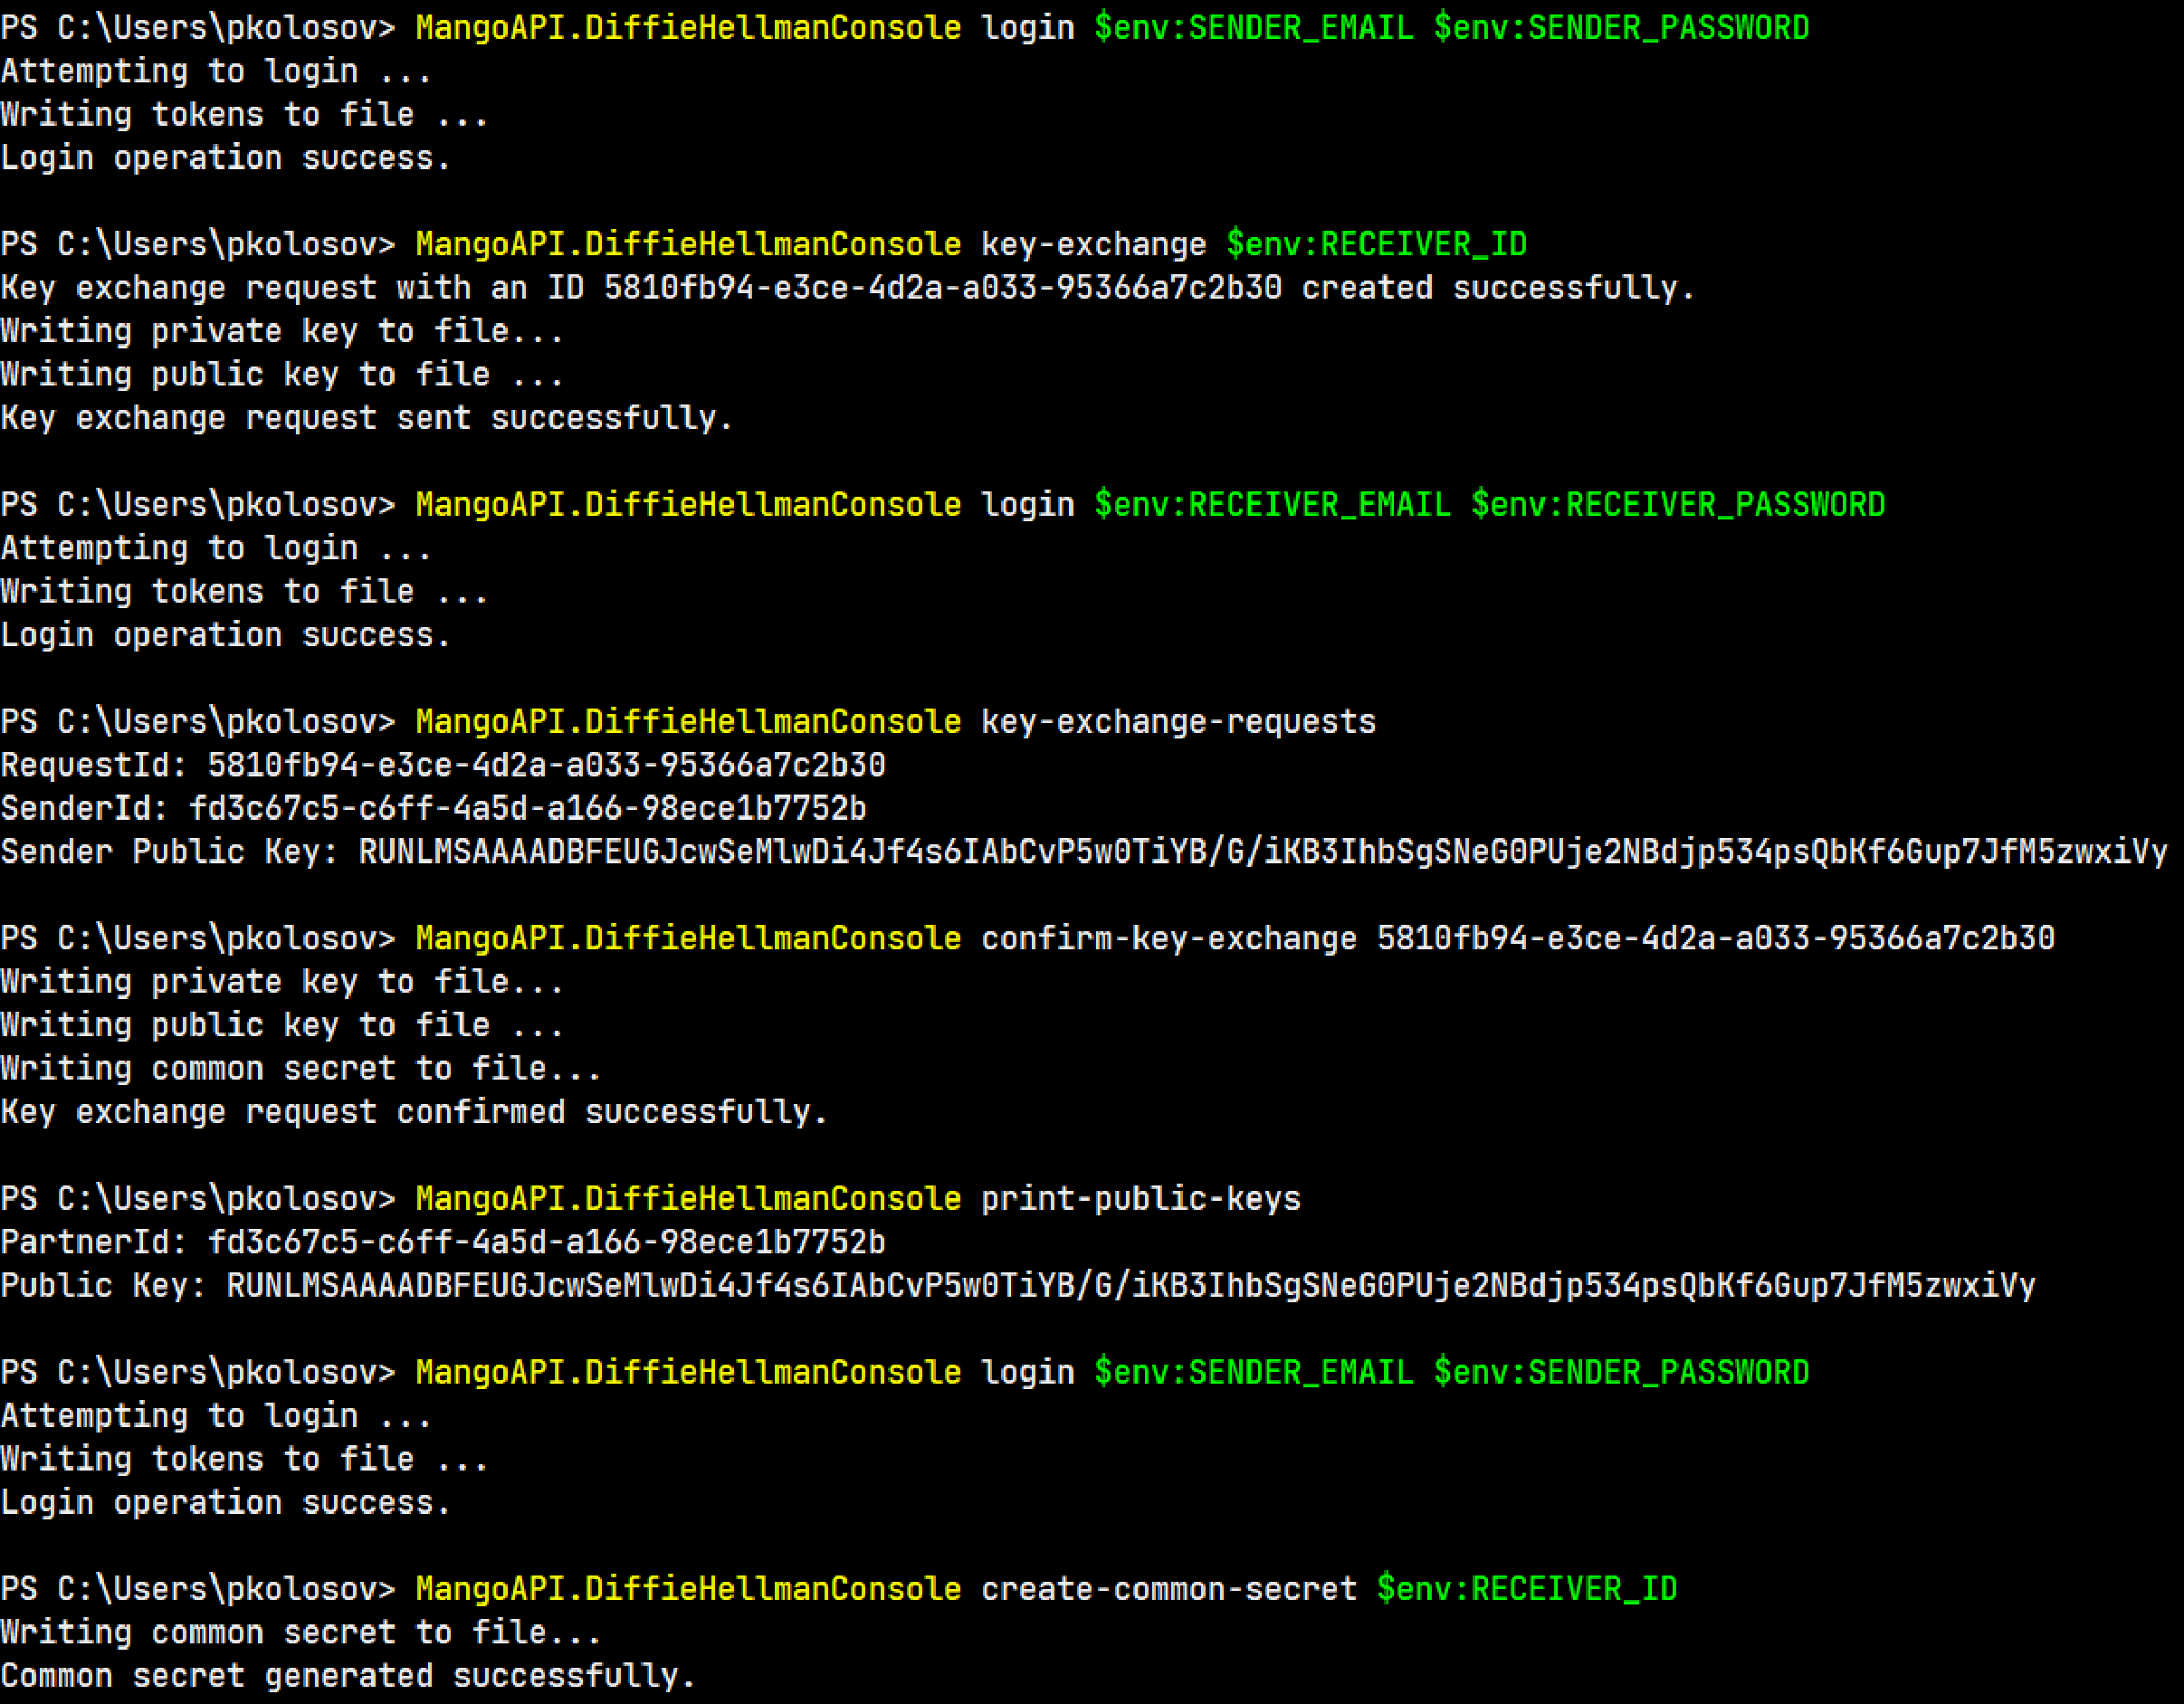
\includegraphics[width=1\textwidth]{Pictures/Diffie_Hellman_console_output}
    ~\caption{Diffie–-Hellman key exchange console output.}\label{fig:figure7}
\end{figure}
In order to repeat the outputs on the screenshot the user may reference to the resources
\begin{itemize}
    \item API: \href{https://back.mangomessenger.company/swagger}{\texttt{https://back.mangomessenger.company/swagger}}
    \item Source: \href{https://github.com/MangoInstantMessenger/MangoMessengerAPI}{\texttt{https://github.com/MangoInstantMessenger/MangoMessengerAPI}}
\end{itemize}
Finally, both test accounts reached the same base 64 common secret.
\begin{figure}[H]
    \centering
    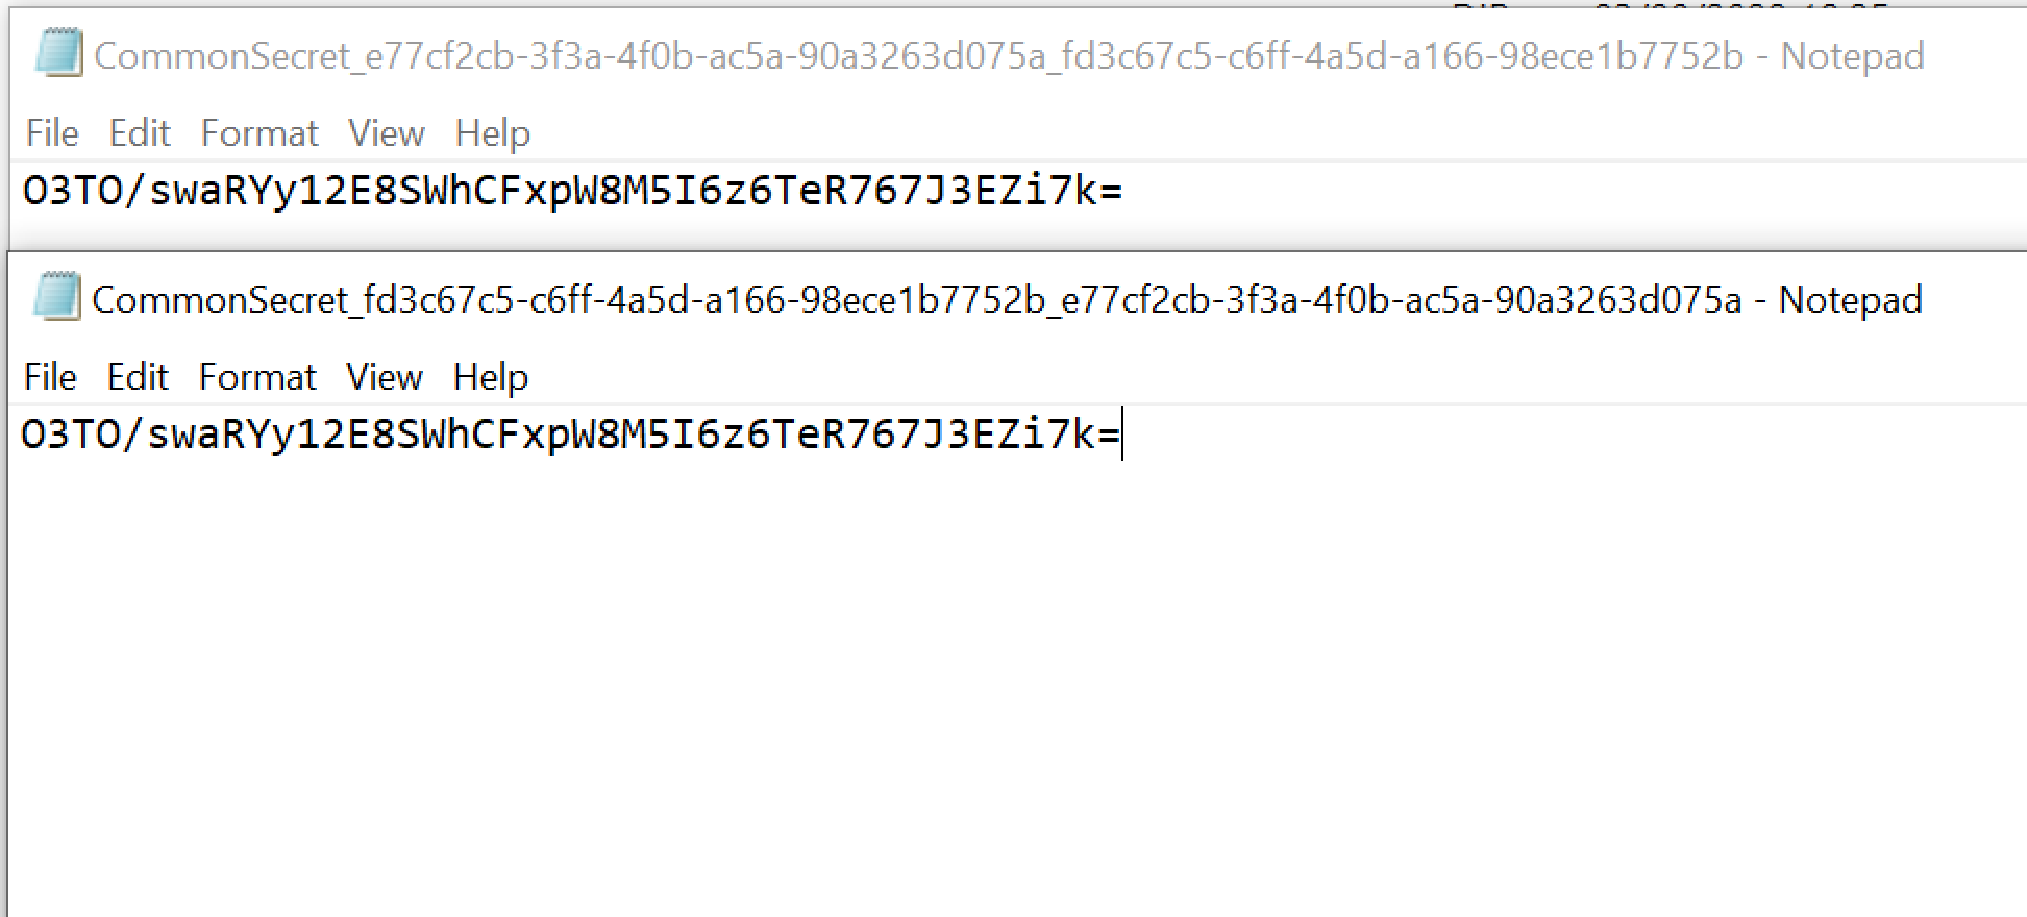
\includegraphics[width=1\textwidth]{Pictures/Same_common_secret}
    ~\caption{Common secrets.}\label{fig:figure2}
\end{figure}